\singlespacing
\chapter{Introducción}
\label{chap:introd}
\spacing{1.5}


\hspace{0.5cm}Desde 1967 hasta la actualidad, la población mundial ha aumentado desde los 3.46 hasta los 7.78 billones de personas. ¿Cómo se va a aumentar la producción de alimentos para alimentar una población mundial estimada para 2050 de 9700 millones de personas? ¿Cómo se va a producir la energía necesaria para dicha población sin comprometer los recursos para las futuras generaciones? ¿Cómo se van a monitorear los recursos naturales de nuestro planeta como los glaciares, los bosques y los ríos?

\begin{figure}[H]
\centering
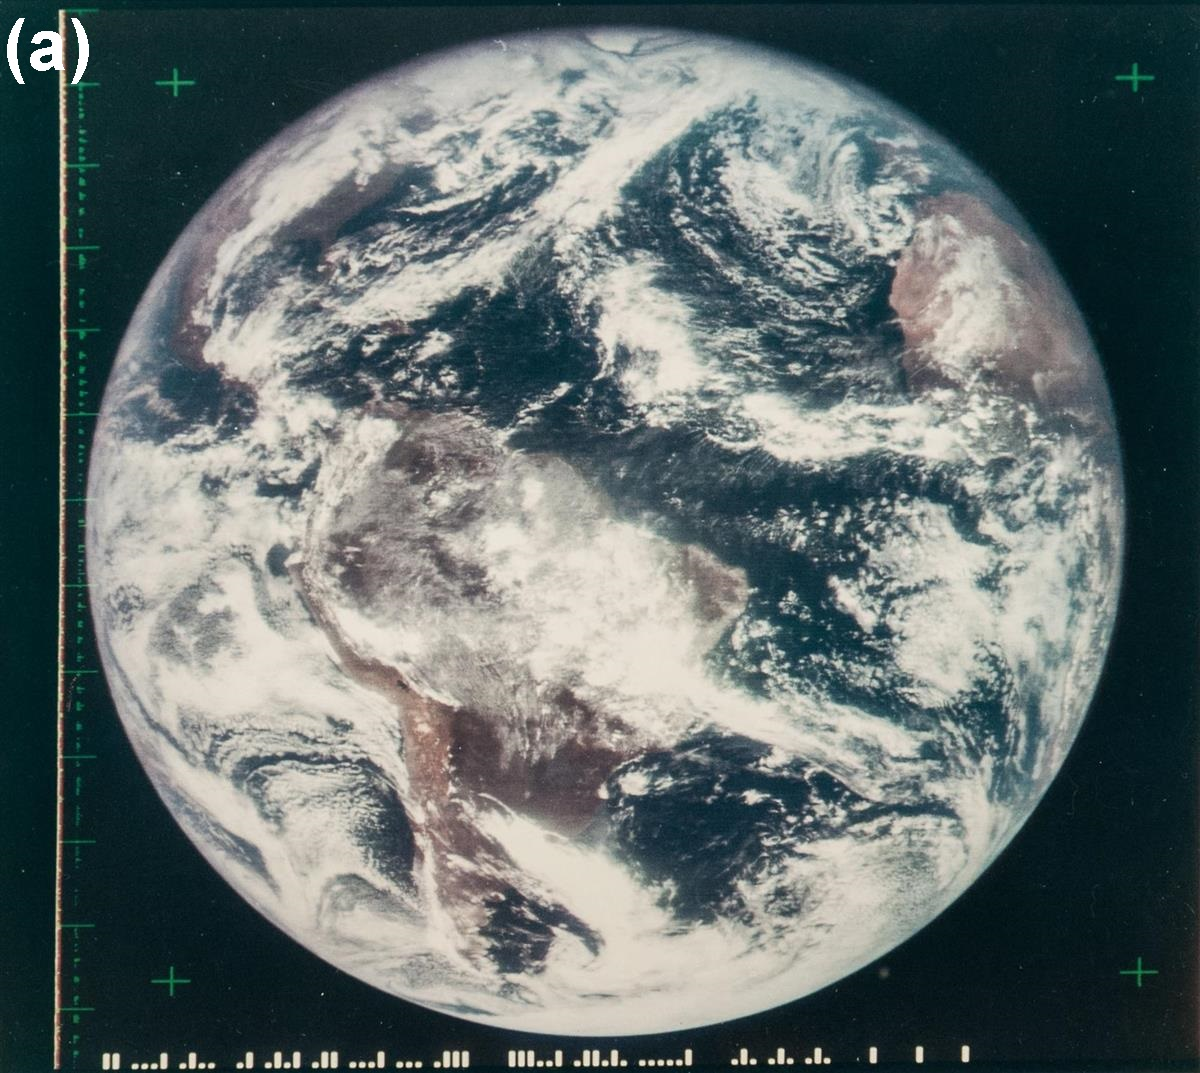
\includegraphics[scale=0.179]{Figs/introduccion/nasaluna7_0.jpg}\hfill
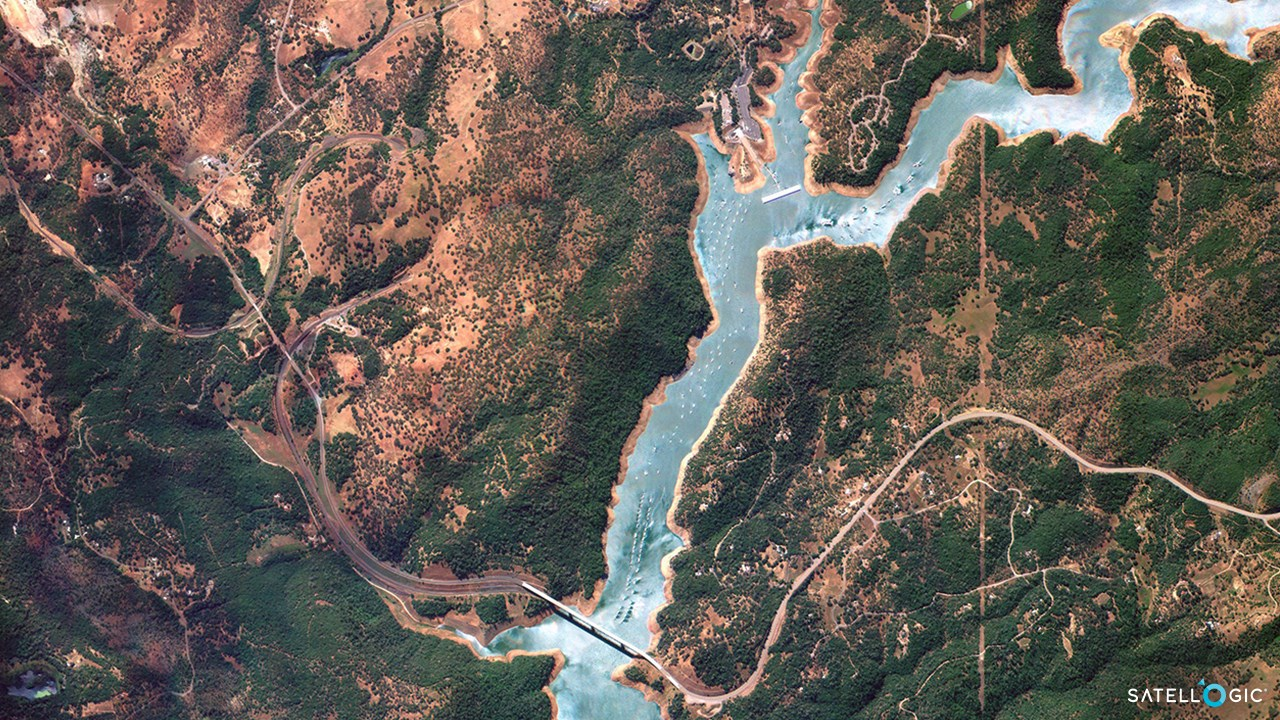
\includegraphics[scale=0.2]{Figs/introduccion/arbolsat.png}
\caption{(a) La primera fotografía en color de todo el planeta Tierra, satélite ATS 3 (10 de noviembre de 1967)  \cite{nattierrra}. (b) Imagen multiespectral de 1 metro de resolución adquirida con una cámara a bordo de uno de los satélites de la compañía Satellogic \cite{imsatt}.}
\label{figs:tierraysatell}
\end{figure}

Una posible respuesta a estos interrogantes puede estar en el entendimiento de la información que nos pueden brindar las imágenes adquiridas por medio de cámaras a bordo de satélites en una constelación de tamaño tal que se pueda obtener una imagen de cada región del planeta con una resolución temporal diaria. Desde la primera adquisición de una fotografía en color de todo el planeta Tierra por una cámara a bordo del satélite ATS 3 en 1967 (Ver Figura \ref{figs:tierraysatell} (a)), la industria satelital se ha desarrollado al punto de que en la actualidad se tiene la posibilidad de adquirir una imagen satelital de 1 metro de resolución espacial que permite identificar y hacer conteo individual de árboles de una región de la Tierra (Ver Figura \ref{figs:tierraysatell} (b)), .

En este capítulo se describe la motivación del proyecto por medio de la explicación del proceso de aquisición de imágenes multiespectrales [\ref{sec:motivacion}] y luego se explica la teoría general detrás del sistema de caracterización de filtros multiespectrales desarrollado en esta tesis [\ref{sec:microespp}].
%%%%%%%%%%%%%%%%%%%%%%%%%%%%%%%%%%%%%%%%%%%%%%%%%%%%%%%%%%%%%%%%%%%%%%%%%%%%%%%%%%%%%%%%%%%%%%%%%%%%%%%%%%%%%%%%%%%%%%%%%%%%%%%%%%%%%%%%%%%%%%%%%%%%%%%%%%%%%%%%%%%%%%%%%%%%%%%%%%%%%%%%%%%%%%%%%%%%%%%%%%%%%%%%%%%%%%%%%%%%

\singlespacing
\section{Adquisición de imágenes multiespectrales}
\label{sec:motivacion}
\spacing{1.5}


\hspace{0.5cm}Una imagen a color RGB convencional está compuesta por tres 
canales de 
imágenes (bandas): rojo 
($\sim$ 665nm), verde ($\sim$ 550nm) y azul ($\sim$ 470nm). Este tipo de 
imágenes permiten emular la percepción que el ojo humano tiene del color, pero 
en general no permiten la detección e identificación de la composición de distintos objetos 
sólidos y 
líquidos, menos 
aún determinar sus propiedades. Para ello 
es necesario obtener información sobre la interacción entre la radiación electromagnética y dichos objetos, es decir sobre el espectro del objeto que permite identificarlo de manera análoga a la identificación de una persona mediante su huella dactilar. Esto último es posible a partir de la captura de imágenes multi e hiperespectrales.

La espectroscopía de imágenes multi e hiperespectrales, en inglés \textit{Multispectral and Hyperspectral Spectroscopy
Imaging} (MSI y HSI, respectivamente), combina la espectroscopía y la adquisición de imágenes en dos dimensiones.
Este método brinda datos espectrales para cada pixel en el campo de visión \footnote{El campo de visión, en inglés \textit{field of view} (FOV), representa el área física de la imagen, que para el caso de una cámara el FOV viene dado por el cociente entre el tamaño del sensor CMOS y la magnificación del microscopio.}. A partir de
dichos datos se puede extraer información sobre la emisión, reflexión ó absorción del objeto de estudio, que puede ser utilizada para determinar su composición físico-química con una cierta
resolución espacial. De esta forma, se pueden identificar tumores de un cáncer \cite{canc}, realizar un
control de calidad de la comida identificando bacterias en tiempo real \cite{food}, optimizar la siembra y la cosecha de ciertos cultivos \cite{cultiv}, monitorear focos de incendios \cite{fire}, entre otras
aplicaciones.

Las imágenes multiespectrales contienen un número acotado de bandas espectrales 
de hasta un par de decenas, con un gran ancho de banda (varias decenas de nm); 
mientras que las hiperespectrales están formadas por un gran número de bandas 
espectrales (de cientos a miles), con una resolución espectral muy estrecha, de 
unos pocos nm (Ver Figura \ref{fig:spectrus}).


\begin{figure}[H]
	\centering
	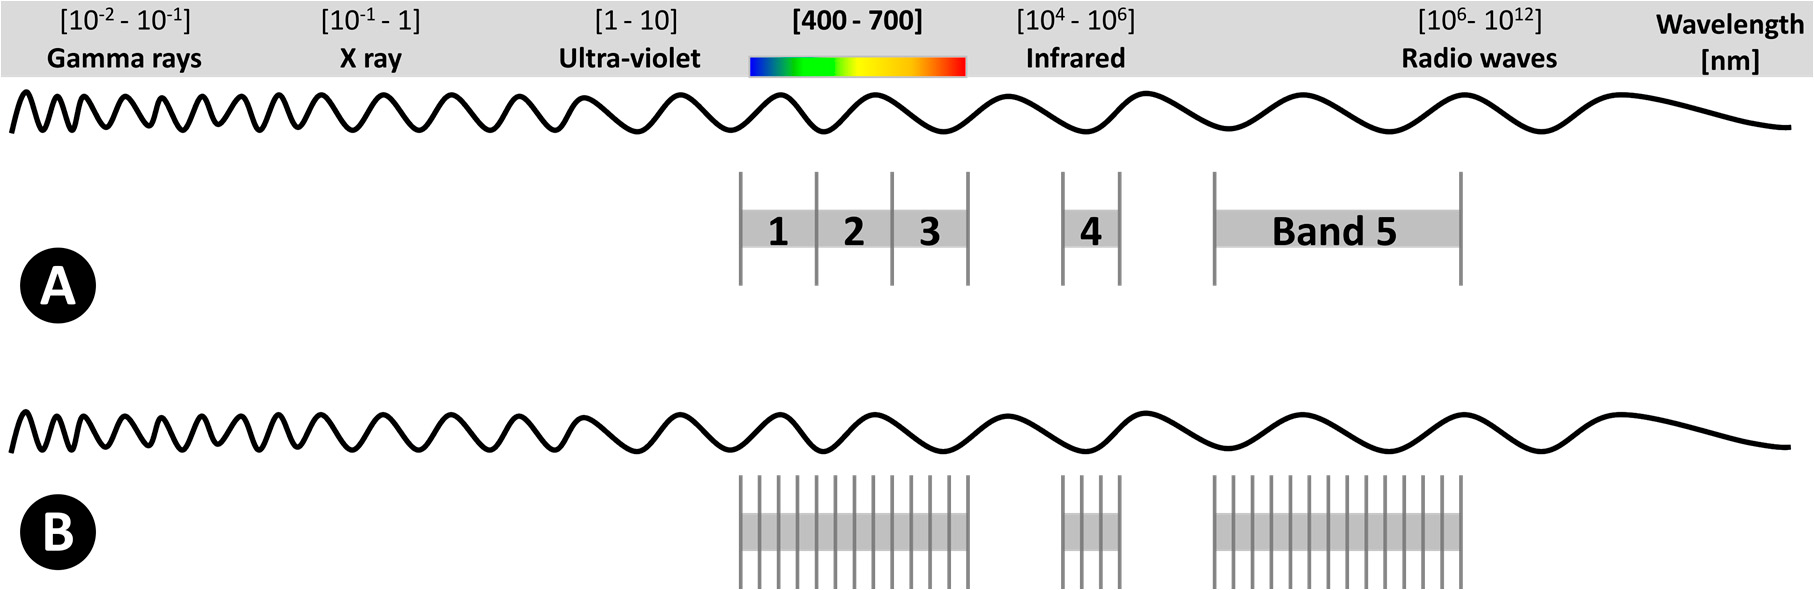
\includegraphics[scale=0.2]{Figs/plan_de_tesis/multivshyper.png}
	\caption{ Representación de los espectros: (A) Multiespectral: 5 
		bandas anchas; y, (B) Hiperespectral: muchas bandas muy estrechas, 
		generalmente entre cientos y miles de ellas. Los dibujos no se 
		encuentran 
		realizados a escala. Imagen adaptada de \cite{Adao2017}.}
	\label{fig:spectrus}
\end{figure}


Las cámaras de adquisición de imágenes multiespectrales estándard utilizan 
redes de difracción o prismas como elementos dispersivos de la luz \cite{5459162}. La 
distancia requerida entre el sensor de detección y el componente de difracción 
de la luz, hace que este tipo de cámaras sean grandes y pesadas\footnote{Por ejemplo, la cámara prismática multiespectral modelo \textit{Fusion Series AD-080CL} del fabricante JAI, tiene una masa de 400 g y unas dimensiones de 55(H) x 55(W) x 80(D) mm \cite{jaii}.}, dos condiciones que en la industria satelital se deben optimizar 
fuertemente ya que el costo de la puesta en órbita de los satélites es 
proporcional a su peso y a su tamaño. Estas cámaras suelen ser caras y 
sensibles a desalinearse debido a las condiciones mecánicas de su construcción. 

En respuesta a las desventajas de las cámaras estándard de imágenes multiespectrales, se desarrollaron otro tipo de cámaras que utilizan filtros de interferencia de banda resultando en un producto final robusto, compacto, 
de bajo costo y de muy buen rendimiento. Una cámara de vuelo de este tipo fue caracterizada en la tesis de licenciatura de Agustina Pose bajo la dirección de Hernán Grecco \cite{Pose2017}. 
Esta cámara tiene la gran ventaja de no presentar partes móviles, 
evitando posibles desalineaciones de los componentes ópticos. Las partes 
móviles de la cámara que serían útiles para realizar un barrido espectral de 
una cierta escena a capturar, no son necesarias pues el barrido es realizado 
por el movimiento propio del satélite respecto de la Tierra. El esquema básico 
de este tipo de 
cámaras multiespectales se muestra 
en la Figura \ref{fig:esquemcamypegfilt} (a), donde una lente enfoca la luz sobre el sensor de imagen que tiene un filtro de múltiples bandas montado arriba de él (Ver Figura \ref{fig:esquemcamypegfilt} (b)).


\begin{figure}[H]
\centering
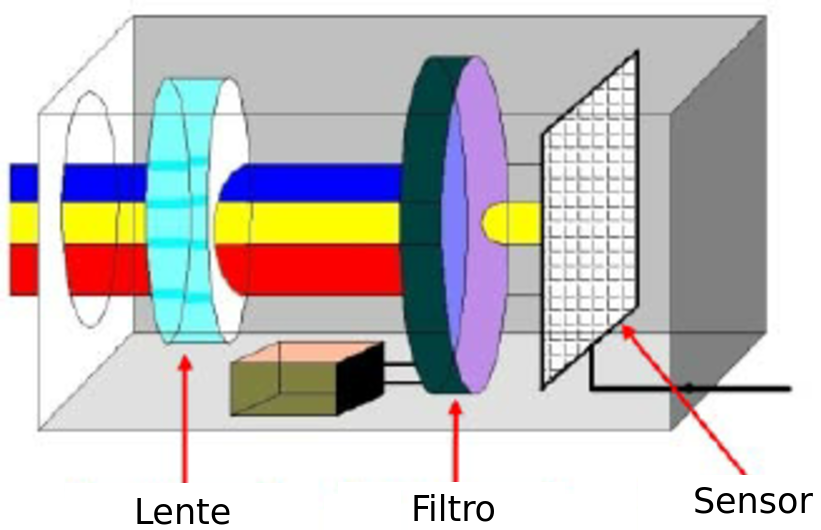
\includegraphics[width=0.5\textwidth]{Figs/plan_de_tesis/cam_sens.png}\hfill
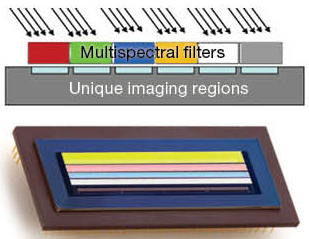
\includegraphics[width=0.5\textwidth]{Figs/introduccion/teled.png}
\caption{(a) Esquema de una cámara multiespectral. El filtro absorbe el espectro completo de la luz incidente salvo la banda espectral que el usuario determina, por lo que sólo las longitudes de onda elegidas atraviesan el filtro y son detectadas por el sensor. Adaptado de \cite{Martinez2008}. (b) Filtro de cinco bandas montado directamente sobre el sensor CCD, es decir en el plano focal del mismo \cite{sensarrib}.}
\label{fig:esquemcamypegfilt}
\end{figure}

 Los filtros de interferencia de banda 
utilizados en este tipo de cámaras deben cumplir ciertos requisitos de calidad como un cierto número, diámetro y tipo de defectos (Ver Capítulo \ref{chap:zeiss}) y ciertas características espectrales y de transmisión (Ver Capítulo \ref{chap:microsp}) antes de ser 
incorporados a la carga útil de, por ejemplo, un satélite que va a ser puesto 
en 
órbita. Esto es así pues dichos filtros se encuentran sobre el plano focal de la imagen por lo que cualquier imperfección del mismo puede repercutir en la calidad de la imagen adquirida. En la Figura \ref{fig:speus} se muestra una imagen multiespectral de cinco bandas cuyas imperfecciones se señalan con círculos rojos. En consecuencia, resulta fundamental caracterizar completamente dichos filtros antes de montarlos sobre las cámaras de los satélites.

\begin{figure}[H]
	\centering
	\includegraphics[width=1.0\textwidth]{Figs/introduccion/0021.png}
	\caption{Imagen multiespectral de cinco bandas, cuyas imperfecciones se señalan con círculos rojos .}
	\label{fig:speus}
\end{figure}

A continuación se realiza una introducción a la teoría detrás del equipo desarrollado en el Capítulo \ref{chap:microsp} que consistió de un microespectrómetro que es un instrumento de medición híbrido que integra la capacidad de magnificación y de resolución ópticas de un microscopio con la capacidad de medir en cada volumen resoluble el espetro de transmisión del filtro.

%%%%%%%%%%%%%%%%%%%%%%%%%%%%%%%%%%%%%%%%%%%%%%%%%%%%%%%%%%%%%%%%%%%%%%%%%%%%%%%%%%%%%%%%%%%%%%%%%%%%%%%%%%%%%%%%%%%%%%%%%%%%%%%%%%%%%%%%%%%%%%%%%%%%%%%%%%%%%%%%%%%%%%%%%%%%%%%%%%%%%%%%%%%%%%%%%%%%%%%%%%%%%%%%%%%%%%%%%%%%

\singlespacing
\section{Microespectroscopía}
\label{sec:microespp}
\spacing{1.5}


\hspace{0.5cm}La microespectroscopía combina la espectroscopía con la microscopía. Existen distintas aplicaciones de esta técnica para estudiar los espectros de muestras microscópicas como la microespectroscopía en el IR (infrarrojo)\cite{WALSH20071}, de FT-IR (\textit{Fourier Transform - Infrared}) \cite{kani}, de Raman \cite{defaria}, etc. En particular en este trabajo se realizaron mediciones de microespectroscopía en el espectro visible y en el cercano infrarrojo (en adelante NIR\footnote{NIR, en inglés \textit{Near-Infrared}, se le denomina a la región espectral del infrarrojo cercano que se extiende aproximadamente desde los 780 nm hasta los 2000 nm.}), en un rango de longitudes de onda comprendido entre los 450 y los 900 nm.

La técnica de microespectroscopía implementada en esta tesis contempla un microscopio de campo brillante integrado con un espectrómetro y una cámara digital como detectores. La microscopía de campo brillante consiste en la generación con un arreglo de lentes de la imagen de una muestra que es iluminada por una fuente de luz. En la Figura \ref{fig:mdb} se muestra el proceso de formación de imágenes de dos puntos (P1 y P2) de una muestra en un microscopio de campo brillante con un objetivo corregido a infinito (O). Se posiciona el objetivo de forma tal que la muestra se encuentre a la distancia focal del mismo. La luz transmitida ó reflejada de la muestra es recolectada y colimada por el objetivo y luego es enfocada por la lente de tubo (en inglés, \textit{tube lens}) en el plano imagen (PI) donde un detector como el espectrómetro ó una cámara pueden ser colocados.

\begin{figure}[H]
	\centering
	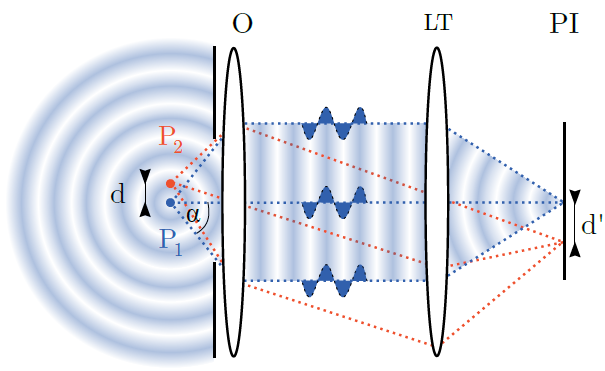
\includegraphics[width=1.0\textwidth]{Figs/introduccion/martinbordenave.png}
	\caption{Proceso de formación de imágenes de dos puntos de una muestra en un microscopio de campo brillante con un objetivo corregido a infinito (O). Adaptado de \cite{borden}.}
	\label{fig:mdb}
\end{figure}

Las características más importantes de un microscopio son su magnificación y el poder de resolución. La magnificación \textit{M} del microscopio que indica la relación entre el tamaño de la imagen y del objeto, viene dada por la siguiente ecuación:
\begin{equation}
M = \frac{f_{LT}}{f_{O}},
\end{equation}	
donde $f_{LT}$ es la distancia focal de la lente de tubo y $f_{0}$ es la distancia focal del objetivo.

El poder óptico de resolución espacial del microscopio estimado teóricamente por el Criterio de Rayleigh viene dado por la siguiente ecuación:
\begin{equation}
d = \frac{0.61 \hspace{2pt} \lambda}{ N.A.},
\end{equation}
donde \textit{d} es la distancia de separación entre los dos puntos de la muestra, $\lambda$ es la longitud de onda de la fuente de luz utilizada y $N.A. = n \hspace{2pt} sin(\alpha)$ es la apertura numérica del objetivo, con $n$ el índice de refracción del medio y $\alpha$ la mitad del ángulo de recolección del objetivo (Ver Figura \ref{fig:mdb}). El criterio de Rayleigh establece que las imágenes de dos fuentes puntuales, incoherentes, de igual intensidad pueden ser, en el límite, distinguidas por un sistema de lentes formador de imágenes, si el centro de uno de los discos de Airy\footnote{Debido a la naturaleza ondulatoria de la luz, las ondas
electromagnéticas interfieren en el plano imagen generando un patrón de intensidad en dos dimensiones con
un máximo en el punto focal, denominado patrón de difracción de Airy \cite{hecht2012optics}.} coincide con el primer mínimo del patrón de Airy de la segunda fuente puntual (Ver Figura \ref{fig:critrayspa}).

\begin{figure}[H]
	\centering
	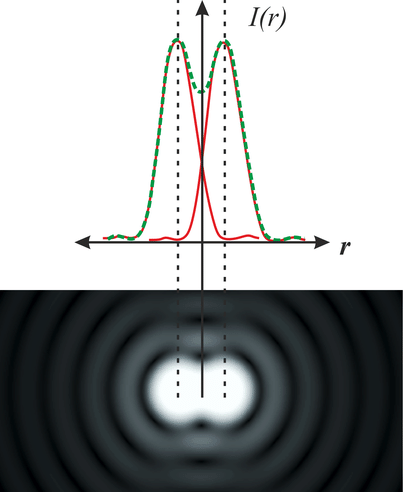
\includegraphics[scale=1.0]{Figs/microespectrometro/raylspa.png}
	\caption{Criterio de Rayleigh para la determinación del límite de resolución. Las curvas rojas representan los patrones de Airy individuales de las dos fuentes puntuales, mientras que la curva verde representa la imagen de las dos fuentes. Las líneas punteadas verticales indican la posición del máximo de cada patrón individual de Airy. Adaptado de \cite{raylsp}.}
	\label{fig:critrayspa}
\end{figure}

La luz que es enfocada por la lente de tubo en el plano imagen es detectada por un espectrómetro en el caso de un microespectrómetro. Para poder aprovechar el poder de resolución óptico del objetivo del microscopio, de acuerdo al Teorema de Nyquist-Shannon se debería utilizar un detector con un área sensible de detección cuyo diámetro sea igual a la mitad del valor de la resolución estimada por Rayleigh. En el caso de una cámara para poder aprovechar la resolución del objetivo cada píxel de la misma debería tener un diámetro equivalente igual a la mitad del valor de la resolución estimada teóricamente. En el caso de un espectrómetro acoplado a una fibra óptica se debe considerar el diámetro del \textit{core} de la misma que guía la luz vía reflexión interna desde el plano imagen (plano de detección) hacia la apertura del espectrómetro.

La fibra óptica es un medio de transmisión de la luz que opera como una guía de ondas dieléctrica cilíndrica por el cual se propaga un único modo si la fibra es monomodo ó múltiples modos si la fibra es multimodo (Ver Figura \ref{fig:guiasmon}). 
\begin{figure}[H]
	\centering
	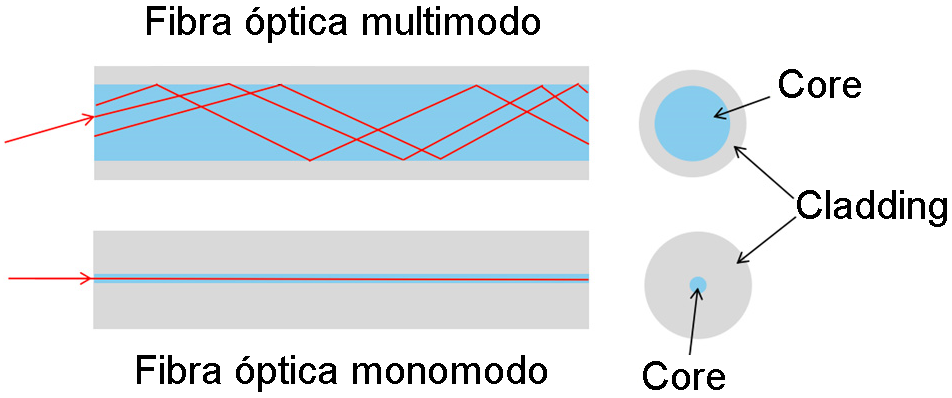
\includegraphics[width=1.0\textwidth]{Figs/introduccion/guias.png}
	\caption{Fibras ópticas mono y multimodo. Adaptado de \cite{dintek}.}
	\label{fig:guiasmon}
\end{figure}
El \textit{core} es la región de la fibra óptica por la cual se realiza la transmisión de la luz y suele estar hecho de vidrio ó de plástico, aunque otros materiales pueden ser utilizados dependiendo del espectro de transmisión deseado. El \textit{cladding} de la fibra que recubre al \textit{core} de la misma, está hecho de un material de las mismas características que el \textit{core} pero con un índice de refracción ligeramente menor (generalmente un 1\% menor)\cite{hecht2012optics}. Esta diferencia en los índices de refracción genera las condiciones para la reflexión total interna dentro de los límites del \textit{core} y a lo largo de la fibra de manera tal que la luz sea transmitida con mínimas pérdidas y no se atenúe a través de las paredes en la frontera con el \textit{cladding}. 

El \textit{core} de la fibra óptica establece una cota para la resolución óptica del microespectrómetro ya que su diámetro establece el valor de la imagen en el plano de la detección y a partir de la magnificación del microespectrómero se puede determinar el tamaño del mínimo objeto detectable. En consecuencia, el diámetro del \textit{core} de la fibra es un parámetro fundamental de diseño del microespectrómetro ya que sólo para determinados diámetros del \textit{core} de la fibra se puede aprovechar el poder de resolución del objetivo con el costo de medir señales de menor intensidad, peor relación señal-ruido y de mayores tiempos de integración de la luz.


%%%%%%%%%%%%%%%%%%%%%%%%%%%%%%%%%%%%%%%%%%%%%%%%%%%%%%%%%%%%%%%%%%%%%%%%%%%%%%%%%%%%%%%%%%%%%%%%%%%%%%%%%%%%%%%%%%%%%%%%%%%%%%%%%%%%%%%%%%%%%%%%%%%%%%%%%%%%%%%%%%%%%%%%%%%%%%%%%%%%%%%%%%%%%%%%%%%%%%%%%%%%%%%%%%%%%%%%%%%%
%%%%%%%%%%%%%%%%%%%%%%%%%%%%%%%%%%%%%%%%%%%%%%%%%%%%%%%%%%%%%%%%%%%%%%%%%%%%%%%%%%%%%%%%%%%%%%%%%%%%%%%%%%%%%%%%%%%%%%%%%%%%%%%%%%%%%%%%%%%%%%%%%%%%%%%%%%%%%%%%%%%%%%%%%%%%%%%%%%%%%%%%%%%%%%%%%%%%%%%%%%%%%%%%%%%%%%%%%%%%
\singlespacing
\section{Organización de la tesis}
\spacing{1.5}

\hspace{0.5cm}En este trabajo de tesis se desarrolló un sistema automatizado de detección y cuantificación de los defectos del filtro. A partir de los resultados de dicha cuantificación se desarrolló un equipo de caracterización de los defectos y de las características espectrales de las bandas del filtro. La tesis está organizada de la siguiente manera.

En el capítulo \ref{chap:zeiss} se define qué es lo que se considera un defecto de un componente óptico [\ref{sec:defectsurf}] y las especificaciones técnicas de las normativas más utilizadas de la industria óptica. Se muestran las características del filtro óptico analizado en el presente trabajo [\ref{sec:carfilt}]. Se explica el proceso de adquisición de imágenes de microscopía [\ref{sec:conf}] del filtro completo y de cada banda espectral. Se muestra el proceso de corrección de la iluminación no uniforme del microscopio [\ref{sec:ilumnou}]  que consistió en la generación de una imagen de fondo [\ref{sec:preproc}] que a su vez fue utilizada para la normalización de las imágenes adquiridas. Asimismo, se detalla el algoritmo utilizado para realizar la detección de los defectos en las imágenes normalizadas [\ref{sec:tthresh},\ref{sec:secalg}]. Se explica la aplicación de los criterios de normas de calidad a los resultados del algoritmo [\ref{sec:resgrl}] y posteriormente se muestran los resultados de caracterización de los defectos denominados huecos. Luego se muestran los resultados de la población de defectos; lo cual permitió establecer los criterios de diseño del microespectrómetro detallado en el Capítulo \ref{chap:microsp}. Finalmente, se explica la asociación de incertezas a los resultados del algoritmo [\ref{sec:incert}].

En el capítulo \ref{chap:microsp} se describe el diseño y la construcción de un microespectrómetro que permitió realizar una caracterización del filtro y de sus defectos a través de los espectros de transmisión. En la Sección \ref{sec:prot0} se muestran las características del primer prototipo desarrollado con equipamiento disponible en el laboratorio. Dicho prototipo en conjunto con los resultados y análisis del Capítulo \ref{chap:zeiss}, permitieron establecer los criterios de elección de la fuente de luz y del espectrómetro, determinar la longitud del recorrido y la precisión mínima necesaria de la platina que se desarrolló y la resolución óptica necesaria del microscopio desarrollado para caracterizar los defectos de diámetro mayores a 20 $\mu m$ de diámetro. Luego se explica el proceso de montaje y alineación preliminar del microespectrómetro. Posteriormente se explica la integración de una cámara \textit{web} al microespectrómetro lo que permitió la adquisición simultánea de imágenes digitales y de espectros de transmisión y cuya área de adquisición fue elegida con un \textit{joystick} y visualizada en vivo a través de una interfaz gráfica. Luego se detalla la caracterización del microespectrómetro [\ref{sec:caractequipo}], su puesta en foco y la determinación de la resolución espacial. Asimismo, se muestra la aplicación del microespectrómetro a la caracterización espectral del filtro y de sus defectos [\ref{sec:resgrales}]. Se describen los resultados de los espectros de transmisión de cada banda del filtro y su comparación con la hoja de datos reportada por el fabricante. Finalmente, se muestran los resultados de la caracterización espectral de los defectos denominados manchas y de los huecos.

Finalmente, en el Capítulo \ref{chap:concls} se describen las conclusiones y las perspectivas de trabajo a futuro.



